\documentclass{article}

\usepackage{amsmath} % For mathematical symbols and environments
\usepackage{amssymb} % For additional mathematical symbols
\usepackage{tcolorbox}
\usepackage{pgfplots} % Add this line to import the pgfplots package

\newtcolorbox{esbox}{
    colback=blue!5!white,
    colframe=blue!75!black,
    fonttitle=\bfseries,
    title=Esempio
}

\title{Definizioni}
\author{Agostino Cesarano}
\date{January 2024}

\begin{document}

\maketitle
\setcounter{part}{4}
\part{Partizione di un intervallo}
Sia $[a,b]$ un intervallo chiuso e limitato. Si dice \textbf{partizione} di
$[a,b]$ un insieme finito di punti $P=\{x_0,x_1,\dots,x_n\}$ tali che
\begin{equation*}
    a=x_0<x_1<\dots<x_n=b
\end{equation*}
\begin{figure}[h]
    \centering
    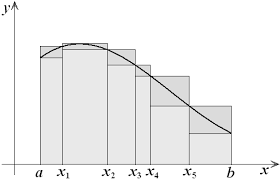
\includegraphics[width=0.5\textwidth]{partizioni.png}
    \caption{Rappresentazione grafica di una partizione}
\end{figure}\\
Ad ogni partizione $[a,b]$ sono associati $n$ intervalli
\[[a,x_1]\cup[x_1,x_2]\cup \dots \cup [x_{n-1},b]=[a,b]\]
Per ogni numero naturale $k \in \{1,\cdots, n\}$, consideriamo il sup e l'inf della funzione f su $[x_{k-1}, x_k]$
\begin{equation*}
    M_k = \sup_{x \in [x_{k-1},x_k]} f(x) \qquad m_k = \inf_{x \in [x_{k-1},x_k]} f(x)
\end{equation*}
$M_k$ e $m_k$ sono rispettivamente l'approssimazione per eccesso e per difetto della funzione $f$ nell'intervallo $[x_{k-1},x_k]$.\\
Definiamo la somma inferiore e la somma superiore della funzione $f$ rispetto alla partizione $P$ come
\begin{equation*}
    S(P,f) = \sum_{k=1}^n M_k(x_k-x_{k-1}) \qquad s(P,f) = \sum_{k=1}^n m_k(x_k-x_{k-1})
\end{equation*}
Naturalmente, $s(P,f) \leq S(P,f)$.
\part{Integrali}
\section*{Integrazione secondo Riemann}
L'integrazione secondo Riemann è un metodo per calcolare l'area sottesa alla curva di una funzione $f(x)$ definita in un intervallo $[a,b]$.\\
Definiamo la somma di Riemann della funzione $f$ rispetto alla partizione $P$ come
\begin{equation*}
    R(P,f) = \sum_{k=1}^n f(\xi_k)(x_{k+1}-x_k)
\end{equation*}
dove $\xi_k \in [x_k,x_{k+1}]$.\\
Se esiste il limite della somma di Riemann per ogni partizione $P$ di $[a,b]$ e se tale limite è indipendente dalla partizione, allora tale limite è detto integrale definito della funzione $f$ in $[a,b]$ e si indica con
\begin{equation*}
    \lim_{\lambda(P) \to 0} R(P,f) = \int_a^b f(x)dx
\end{equation*}
$\lambda(P)$ è la norma della partizione P, ovvero il massimo della lunghezza degli intervalli che compongono la partizione.\\\\
Quindi prese partizioni sempre più piccole dell'intervallo $[a,b]$, la somma di Riemann tenderà ad un valore limite, che è l'area sottesa alla curva della funzione $f(x)$ nell'intervallo $[a,b]$.\\\\

\textbf{Primitiva di una funzione}\\
Sia $f(x)$ una funzione definita in un intervallo $I$. Si dice che $F(x)$ è una primitiva di $f(x)$ in $I$ se $F'(x)=f(x)$ per ogni $x \in I$.\\\\
\textbf{Formula fondamentale del calcolo integrale}\\
Sia $f(x)$ una funzione continua in $[a,b]$. Sia $F(x)$ una primitiva di $f(x)$ in $[a,b]$. Allora
\begin{equation*}
    \int_a^b f(x)dx = F(b)-F(a)
\end{equation*}
\section*{Proprietà degli integrali}
Sia $f(x)$ una funzione continua in $[a,b]$. Allora $f(x)$ è integrabile in $[a,b]$.\\\\
\textbf{Additività}\\
Se a, b e c sono tre numeri reali tali che $a \leq b \leq c$ e se $f(x)$ è una funzione continua in $[a,c]$, allora
\begin{equation*}
    \int_a^c f(x)dx = \int_a^b f(x)dx + \int_b^c f(x)dx
\end{equation*}
\textbf{Linearità}\\
Se $f(x)$ e $g(x)$ sono due funzioni continue in $[a,b]$ allora
\begin{equation*}
    \int_a^b (f(x)+g(x))dx = \int_a^b f(x)dx + \int_a^b g(x)dx
\end{equation*}
Se $f(x)$ è una funzione continua in $[a,b]$ e se $c \in \mathbb{R}$, allora
\begin{equation*}
    \int_a^b cf(x)dx = c\int_a^b f(x)dx
\end{equation*}
\textbf{Modulo}\\
Se $f(x)$ è una funzione continua in $[a,b]$, allora
\begin{equation*}
    \left|\int_a^b f(x)dx\right| \leq \int_a^b |f(x)|dx
\end{equation*}
\textbf{Monotonia}\\
Siano $f(x)$ e $g(x)$ due funzioni continue in $[a,b]$. Se $f(x) \leq g(x)$ per ogni $x \in [a,b]$, allora
\begin{equation*}
    \int_a^b f(x)dx \leq \int_a^b g(x)dx
\end{equation*}
\textbf{Osservazioni}\\
Sia $f(x)$ una funzione continua in $[a,b]$. Allora
\begin{equation*}
    \int_a^b f(x)dx = -\int_b^a f(x)dx
\end{equation*}
\begin{equation*}
    \int_a^a f(x)dx = 0
\end{equation*}
Se gli estremi di integrazione sono uguali, l'integrale è nullo.\\\\
\section*{Integrali indefiniti}
Sia $f(x)$ una funzione continua in un intervallo $[a,b]$. L'insieme delle primitive di $f(x)$ in $[a,b]$ è dato da
\begin{equation*}
    \int f(x)dx=F(x)+c
\end{equation*}
Dove $c \in \mathbb{R}$ è una costante arbitraria.\\
%Integrali immediati%
\section*{Integrali immediati}
\begin{itemize}
    \item $\int x^pdx = \frac{x^{p+1}}{p+1}+c \qquad p \neq -1$
    \item $\int \frac{1}{x}dx = \ln|x|+c \qquad x>0$
    \item $\int e^xdx = e^x+c$
    \item $\int \sin xdx = -\cos x+c$
    \item $\int \cos xdx = \sin x+c$
    \item $\int \frac{1}{\cos^2x}dx = \tan x+c$
    \item $\int \frac{1}{1+x^2}dx = \arctan x+c$
\end{itemize}
\textbf{Integrazione di funzioni razionali fratte}\\
Si supponga di dover integrare una funzione razionale fratta del tipo
\begin{equation*}
    \int \frac{P(x)}{Q(x)}dx
\end{equation*}
dove $P(x)$ e $Q(x)$ sono polinomi.\\
Se il grado di $P(x)$ è maggiore o uguale al grado di $Q(x)$, si divide $P(x)$ per $Q(x)$ e si ottiene
\begin{equation*}
    \frac{P(x)}{Q(x)} = K(x) + \frac{R(x)}{Q(x)}
\end{equation*}
dove $K(x)$ è un polinomio e $R(x)$ è un polinomio di grado minore di $Q(x)$.\\
Si può quindi scrivere
\begin{equation*}
    \int \frac{P(x)}{Q(x)}dx = \int K(x)dx + \int \frac{R(x)}{Q(x)}dx
\end{equation*}
L'integrale del primo termine è immediato, mentre per il secondo termine si procede con la decomposizione in fratti semplici.\\\\
Se il grado di $P(x)$ è minore del grado di $Q(x)$, si procede con la decomposizione in fratti semplici.\\\\
\textbf{Decomposizione in fratti semplici}\\
Sia $P(x)$ un polinomio di grado $n$ e sia $Q(x)$ un polinomio di grado $m$ con $n<m$.\\\\
Se $\Delta = b^2-4ac > 0$, allora $Q(x)$ ha due radici reali distinte.\\
\begin{equation*}
    \frac{P(x)}{Q(x)} = \frac{A}{x-a} + \frac{B}{x-b}
\end{equation*}
%Integrale che si ottiene%
\begin{equation*}
    \int \frac{P(x)}{Q(x)}dx = A\ln|x-a|+B\ln|x-b|+c
\end{equation*}
Se $\Delta = b^2-4ac = 0$, allora $Q(x)$ ha due radici reali coincidenti.\\
\begin{equation*}
    \frac{P(x)}{Q(x)} = \frac{A}{x-a} + \frac{B}{(x-a)^2}
\end{equation*}
%Integrale che si ottiene%
\begin{equation*}
    \int \frac{P(x)}{Q(x)}dx = A\ln|x-a|+B\frac{1}{x-a}+c
\end{equation*}
Se $\Delta = b^2-4ac < 0$, allora $Q(x)$ ha due radici complesse coniugate.\\\\
%Si dividono in due casi%
Numeratore di grado 1 e denominatore di grado 2\\
\begin{equation*}
    \frac{P(x)}{Q(x)} = \frac{lx+a}{ax+bx+c} = \frac{A(2ax+b)}{ax^2+bx+c}+\frac{B}{ax^2+bx+c}
\end{equation*}
%Integrale che si ottiene%
\begin{equation*}
    \int \frac{P(x)}{Q(x)}dx = A\ln|ax^2+bx+c|+B\arctan\left(\frac{2ax+b}{\sqrt{4ac-b^2}}\right)+c
\end{equation*}
Numeratore di grado 0 e denominatore di grado 2\\
\begin{equation*}
    \frac{P(x)}{Q(x)} = \frac{A}{ax^2+bx+c}
\end{equation*}
%Integrale che si ottiene%
\begin{equation*}
    \int \frac{P(x)}{Q(x)}dx = \frac{A}{\sqrt{4ac-b^2}}\arctan\left(\frac{2ax+b}{\sqrt{4ac-b^2}}\right)+c
\end{equation*}
Se $x^2+bx+q$ è irriducibile, allora
\begin{equation*}
    \frac{P(x)}{Q(x)} = \frac{Ax+B}{x^2+bx+c} = \frac{Ax+B}{(x+\alpha)^2+\beta^2}
\end{equation*}
dove $\alpha = -\frac{b}{2}$ e $\beta = \frac{\sqrt{b^2-4c}}{2}$.\\\\
%Integrale che si ottiene%
\begin{equation*}
    \int \frac{P(x)}{Q(x)}dx = A\arctan\left(\frac{x+\alpha}{\beta}\right)+B\ln|(x+\alpha)^2+\beta^2|+c
\end{equation*}
\newpage
\section*{Integrazione per sostituzione}
Sia $f(x)$ una funzione continua in un intervallo $I$. Sia $g(x)$ una funzione derivabile in $I$.\\
Se $f(x)$ è della forma $f(g(x))g'(x)$, allora
\begin{equation*}
    \int f(g(x))g'(x)dx = \int f(t)dt
\end{equation*}
dove $t=g(x)$.\\\\
\begin{itemize}
    \item Capire quale funzione $g(x)$ può essere utile per semplificare l'integrale.
    \item Calcolare la derivata di $g(x)$.
    \item Sostituire $t=g(x)$ e $dx=g'(t)dt$.
    \item Sostituire $f(g(x))g'(x)dx$ con $f(t)dt$.
    \item Nel caso in cui l'integrale sia definito, sostituire gli estremi di integrazione.
\end{itemize}
\section*{Integrazione per parti}
Siano $f(x)$ e $g(x)$ due funzioni derivabili in un intervallo $I$.\\
Allora
\begin{equation*}
    \int f(x)g'(x)dx = f(x)g(x) - \int f'(x)g(x)dx
\end{equation*}
\begin{itemize}
    \item Scegliere $f(x)$ e $g'(x)$.
    \item Calcolare $f'(x)$ e $g(x)$.
    \item Sostituire $f(x)g'(x)dx$ con $f(x)g(x)-\int f'(x)g(x)dx$.\\\\
\end{itemize}
\end{document}